\documentclass[a4j,10pt]{jarticle}
\usepackage[dvipdfm,text={160mm,240mm},centering]{geometry}
\usepackage{newtxtext,newtxmath}
\usepackage[dvipdfmx]{graphicx}
\usepackage{listings,jvlisting}
\usepackage{color}
\usepackage{tabularx}
\usepackage{booktabs}
\usepackage{multirow}
\usepackage[framemethod=tikz]{mdframed}

% 担当教員名
\newcommand{\teacherName}{桝井 晃基}
% 提出者名
\newcommand{\studentName}{鶴見 俊介}
% 提出者所属
\newcommand{\studentAff}{基礎工学部 情報科学科3年 計算機科学コース}
% 提出者学籍番号
\newcommand{\studentID}{09B23057}
% 提出者電子メールアドレス
\newcommand{\studentEmail}{u299151f@ecs.osaka-u.ac.jp}
% 課題提出日
\newcommand{\submitted}{\today}
% 課題締め切り日
\newcommand{\deadline}{2025年11月14日}

\lstset{
    basicstyle = {\ttfamily},
    backgroundcolor  = {\color[gray]{.99}},
    breaklines = true,
    columns = [l]{fullflexible},
    commentstyle = {\smallitshape},
    frame = {tb},
    identifierstyle = {\small},
    keepspaces=true,
    keywordstyle = {\small\bfseries},
    lineskip = -0.5ex,
    ndkeywordstyle = {\small},
    numbers = left,
    numbersep = 1zw,
    numberstyle = {\scriptsize},
    stepnumber = 1,
    stringstyle = {\small\ttfamily},
    xleftmargin = 3zw,
    xrightmargin = 0zw
}
\renewcommand{\lstlistingname}{プログラム}

\begin{document}
\begin{titlepage}
\begin{center}
{\Huge\bfseries 情報科学演習D} \\
\vspace{1cm}
{\LARGE\bfseries 課題2}
\vspace{5cm}

{\large
\begin{tabular}{rcl}
担当教員 & : & \teacherName \\
提出者   & : & \studentName \\
所属/学年   & : & \studentAff\\
学籍番号 & : & \studentID \\
電子メール & : & \texttt{\studentEmail}\\
&& \\
提出日 & : & \submitted \\
締切日 & : & \deadline
\end{tabular}
}
\end{center}
\end{titlepage}

\setcounter{tocdepth}{2}
% \tableofcontents
\newpage

% \lstinputlisting[caption=サーバプログラムの接続手順, firstline=1, firstnumber=1, lastline=19, label=prog:server]{codes/server.txt}


\section{システムの仕様}
\verb|Pascal|風言語で記述されたプログラムのトークン列ファイル（\verb|ts|ファイル）を第一引数として入力し，プログラムの構文が正しいかどうか判定する構文解析プログラムを作成する．
構文が正しい場合は文字列 \verb|"OK"| を返し，構文が正しくない場合は文字列 \verb|"Syntax error: line"| という文字列とともに，最初の誤りを見つけた行番号を返す．
入力ファイル内に複数の誤りが含まれる場合は，最初に見つけた誤りの行番号のみ返す．
また，入力ファイルが見つからない場合は，文字列 \verb|"File not found"| を返す．

なお，本構文解析器は構文が正しいと判定できた場合に限り，後続の意味解析に用いるための抽象構文木（\verb|AST|）を内部に構築する（根は \verb|Program|，主な子は \verb|Block| と \verb|Compound| 等）．
各 \verb|AST| ノードは少なくとも種別と先頭・末尾行の位置情報を保持する．
エラー検出時は解析を中止するため，\verb|AST| は確定しない．

\section{課題達成の方針と設計}
\subsection{中核アイデアと設計原則}
本実装は，字句解析済みトークン列を入力とし，トップダウンの再帰下降型で構文木（\verb|AST|）を生成する．
文・宣言・式などの各非終端記号の解析は，それぞれ\verb|parseStmt()|, \verb|parseDecl()|, \verb|parseExpr()| のような関数に対応付け，規則=関数の直観的な呼び出し構造を採る．

構文解析は，左再帰性を含まない無曖昧な文法で，1トークンの先読み（\verb|LL(1)|）を用いる．
指導書の\verb|EBNF|は，文と基本文の分岐先決定に2トークンの先読み（\verb|LL(2)|）が必要なため，\verb|LL(1)|で解析可能な文法に修正する必要がある．
実装は \verb|peek()|による定数回の確認で解決し，バックトラックは行わないことで決定性と線形時間性を維持する．

また，構文解析を進めながら，トークン列を木構造に保存して\verb|AST|を作成していく．
\verb|AST|の作成は，構文解析においては必須ではないが，後の意味解析以降の処理で再利用可能な形となることに加え，軽量で後続の処理と疎結合となり拡張性をもつメリットがあると考えられる．

以上により，文法の明確化（左再帰除去と先読み設計）と実装の単純性（関数と規則の対応，決定的分岐），および将来拡張性（\verb|AST|中心設計）を同時に満たす方針とした．


\subsection{データ構造}
\begin{figure}[h]
  \centering
  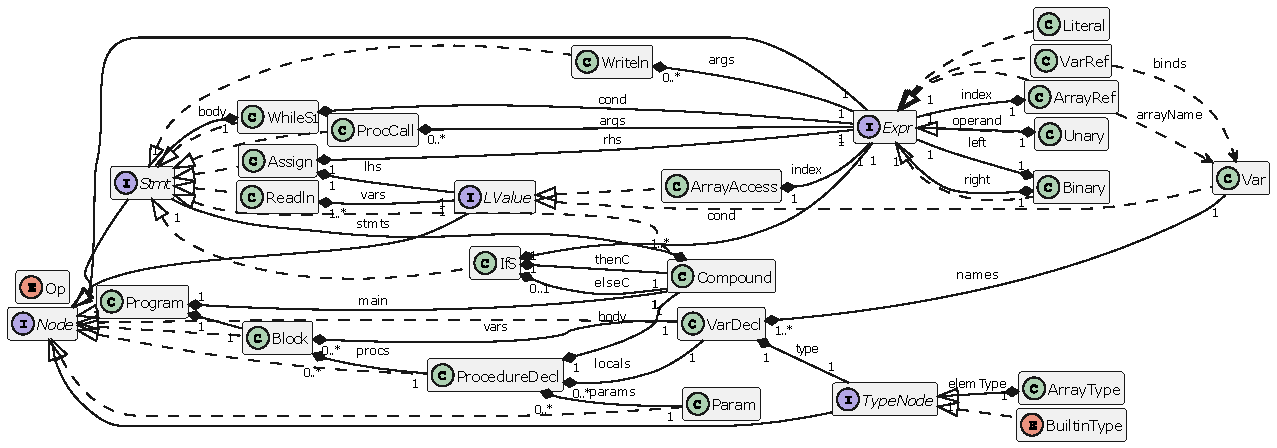
\includegraphics[width=1.05\linewidth]{images/ast/ast-2.pdf}
  \caption{ASTのクラス図}
  \label{fig:ast}
\end{figure}

まず，\verb|TsSource|が入力ファイル内文字列の各行を，名前・トークン種・トークン\verb|ID|・行番号の4つの要素に分解して，\verb|TsToken|型の\verb|List|に順に格納していくことで，トークンに関する情報は保存される．
このようにして保存された\verb|List|を順に参照していくことで構文解析を行い，\verb|AST|を作成していく．

本課題の\verb|AST|は，\verb|Node| を共通基底とする木構造であり，各ノードは種別，子ノード，行番号をもつ．
種別は，構造系（\verb|Program|・\verb|Block|・\verb|Compound|），
宣言系（\verb|VarDecl|・\verb|ProcedureDecl|・\verb|Param|・\verb|ArrayType|・\verb|BuiltinType|），
文系（\verb|Assign|・\verb|IfS|・\verb|WhileS|・\verb|ProcCall|・\verb|Readln|・\verb|Writeln|），
式系（\verb|Binary|・\verb|Unary|・\verb|Literal|・\verb|VarRef|・\verb|ArrayRef|）に大別する．
左辺値 は \verb|LValue| として抽象化し，\verb|Var| と \verb|ArrayAccess| が実装する．
演算子種別は \verb|Op| 列挙で保持し，優先順位・結合性は木構造（例：\verb|Binary(op=ADD, left=..., right=...)|）に反映する．
これらの木構造のクラス関係をまとめたものが図\ref{fig:ast}である．


\subsection{解析アルゴリズム}

\begin{figure}[h]
  \centering
  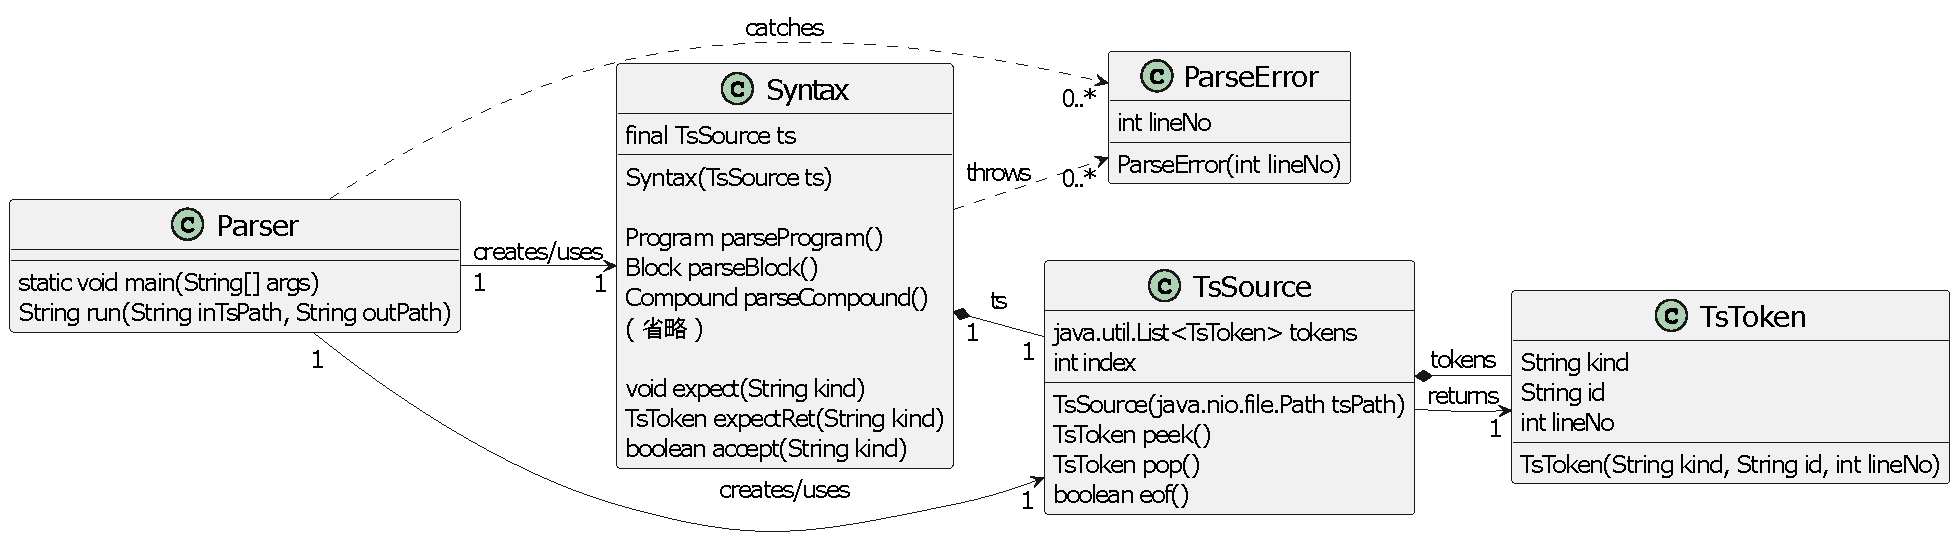
\includegraphics[width=\linewidth]{images/parser/parser.pdf}
  \caption{構文解析のクラス図}
  \label{fig:parser}
\end{figure}

\begin{figure}[h]
  \centering
  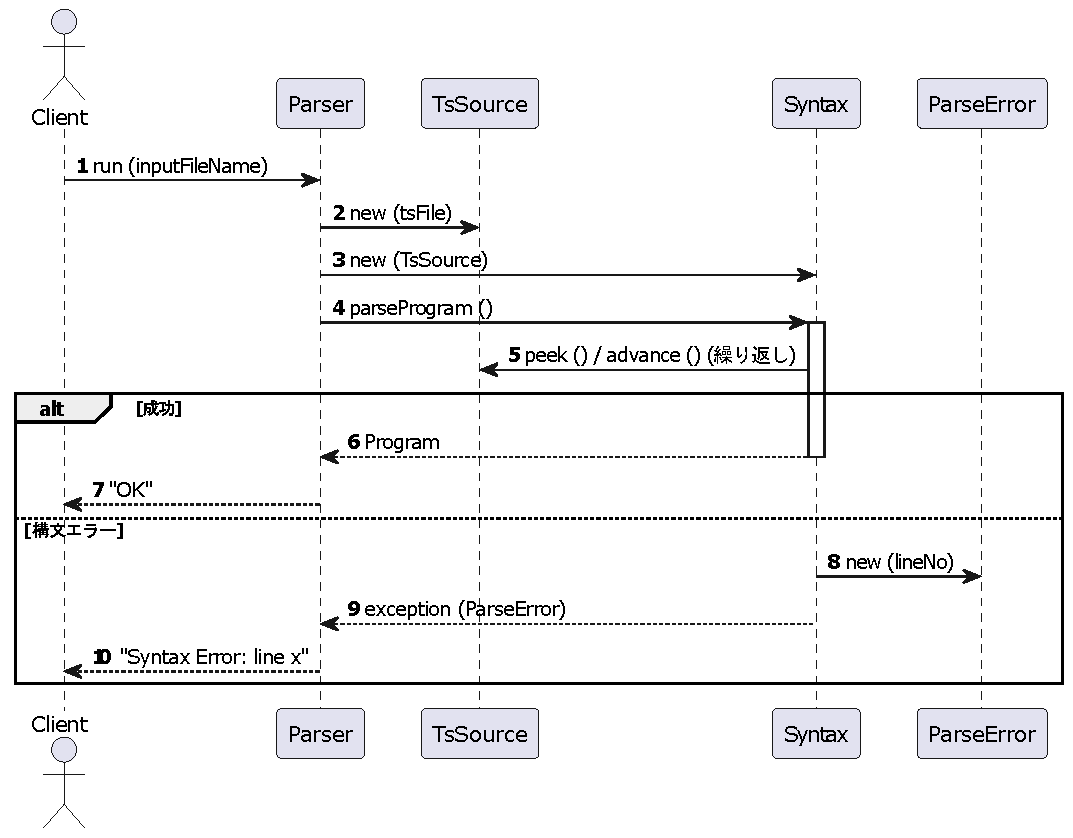
\includegraphics[width=0.81\linewidth]{images/sequence/sequence.pdf}
  \caption{構文解析のシーケンス図}
  \label{fig:sequence}
\end{figure}

図\ref{fig:parser}は全体の処理におけるクラス間の関係を表したクラス図であり，図\ref{fig:sequence}はそれらのクラスが処理を行う流れを表したシーケンス図である．
これらによる呼び出し関係と処理の流れをまとめると次にようになる．
なお，以下の処理番号は図\ref{fig:sequence}中の番号と対応している．

\begin{enumerate}\setlength{\itemsep}{0pt}
  \item \verb|Client| が \verb|Parser.run(inputFileName)| を起動する．
  \item \verb|Parser| は入力TSファイルから \verb|TsSource| を生成する．
  \item \verb|Parser| は \verb|TsSource| を引数に \verb|Syntax| を生成する．
  \item \verb|Parser| は \verb|Syntax.parseProgram()| を呼び出し，解析を開始する．
  \item \verb|Syntax| は \verb|TsSource.peek()/advance()| を繰り返し用いてトークンを消費し，対応する \verb|AST| を構築する．
        解析が成功したら6へ，失敗したら8へ進む．
  \item \verb|Syntax| は \verb|Program| ノードを \verb|Parser| に返す．
  \item \verb|Parser| は \verb|"OK"| を \verb|Client| に返して終了する．
  \item \verb|Syntax| は \verb|ParseError(lineNo)| を生成する．
  \item \verb|Syntax| は \verb|Parser| に例外 \verb|ParseError(lineNo)| を送出する.
  \item \verb|Parser| は \verb|"Syntax Error: line x"| を \verb|Client| に返して終了する．
\end{enumerate}






\section{実装プログラム}
全体の処理は図\ref{fig:sequence}の流れによって行われるが，この内の\verb|Parser|が\verb|Syntax.parseProgram()|を呼び出すことで構文解析を開始する．
以下のプログラム\ref{prog:parseProgram}は，\verb|parseProgram()|の実装内容である．
\verb|parseProgram()|は，\verb|「プログラム = "program" プログラム名 ";" ブロック 複合文 "."」|という順番で記述されているかどうかを検査する．
以降は「非終端＝関数」の対応で，上位規則から下位規則へ決定的に遷移する．
ここで呼び出されている関数\verb|expect(String)|は引数で渡された文字列がトークン名と一致しているかどうかを判定し，一致しているならばトークンを消費，一致していないならば例外\verb|ParseError|を送出する．
\verb|expectRet(String)|は引数で渡されたトークン種と一致しているかどうかを判定し，一致しているならばそのトークンを返す\verb|TsToken|型の関数であり，一致しないならば例外\verb|ParseError|を送出する．

また，プログラムはブロックと複合文を構成要素としているが，これらも同様に文法的に正しく記述されているか確認する必要がある．
\verb|parseBlock()| は宣言列，\verb|parseCompound()| は \verb|Stmt| の1個以上の並びを担当する．
これらの関数も\verb|parseProgram|と同様に，各非終端の検査に対応した関数を呼び出す．
各関数は期待されるトークン列を \verb|expect| などで検証・消費しながら対応する \verb|AST| ノードを生成し，復帰時に親子関係を確定する．

以上を各規則に対して再帰的に適用することで，図\ref{fig:sequence}の流れに沿って入力全体を一意に解析し，最終的に \verb|Program| を根とする \verb|AST| を得る．


\lstinputlisting[caption=parseProgram, firstline=1, firstnumber=1, lastline=9, label=prog:parseProgram]{codes/parseProgram.txt}




\section{考察や工夫点}
\subsection{EBNFによる生成規則}
指導書の\verb|EBNF|を修正して，\verb|LL(1)|で解析が可能になるような文法を作成した．
これによって，\verb|LL(2)|によるバックトラックが生じることなく構文解析を完了することができる．

修正した部分は，基本文と文の生成規則である．
基本文は，「基本文 = 代入文｜手続き呼出し文｜入出力文｜複合文」として定義されているが，代入文と手続き呼び出し文はともに先頭が識別子であるため，先頭トークンが識別子だった場合に分岐先が確定しない．
したがって，以下のように非終端「代入または手続き」を追加して1トークンの先読みで解析ができるようにする．

\begin{mdframed}[roundcorner=4pt, linewidth=0.6pt, innertopmargin=4pt, innerbottommargin=4pt, innerleftmargin=20pt]
基本文 = 識別子 \textbf{代入または手続き}｜入出力文｜複合文\\
\textbf{代入または手続き} = \verb|":=" 式｜[ "(" 式の並び ")" ]|
\end{mdframed}

同様に，文の生成規則における\verb|if文|への分岐も，\verb|else|の有無が1トークンの先読みでは確定しない文法になっているため，次のように非終端「\verb|else|文」を追加して修正する．
\begin{mdframed}[roundcorner=4pt, linewidth=0.6pt, innertopmargin=4pt, innerbottommargin=4pt, innerleftmargin=20pt]
文 = 基本文｜\verb|"if" 式 "then" 複合文|\hspace{8pt}\textbf{else文} \verb|｜"while" 式 "do"| 複合文\\
\textbf{else文} = \verb|[ "else" 複合文 ]|
\end{mdframed}

また，左再帰性を含む生成規則も\verb|LL(1)|での解析が不能である．
指導書の\verb|EBNF|には左再帰性は含まれていないが，「\verb|E→E+T｜T|」のようにして含まれていた場合は，「\verb|E→TE'|」「\verb|E'→ε｜+TE'|」のようにして左再帰性を除去する必要がある．
なぜならば，「\verb|E→E+T｜T|」のように左再帰性があると，\verb|First(E)=First(T)|となり，\verb|E|の分岐先が1トークンの先読みでは確定せず，\verb|E→E+T|の生成を無限に選択してしまうためである．
このように，\verb|LL(1)|による簡潔な解析を実装するためには，左因子分解と左再帰性除去による無曖昧な文法が必要であるとわかる．

\subsection{ASTの役割・将来性}
\verb|AST| はプログラムの構文構造を失わずに最小情報で表す中間表現である．
文法規則を木に写像することで，整形出力・可視化・回帰テストの基盤になり，将来の意味解析やコード生成を疎結合に追加できる．
一方で属性を増やしすぎると重くなるため，今回の最小設計（種別・子列・位置）に抑えた判断は妥当だと考える．
構文解析の段階では \verb|AST| の利点は限定的だが，\verb|Visitor| パターン等により後続機能（ダンプ整形，静的検査，IR生成）の拡張余地が確保できた点は大きい．


\section{感想}
今回の実装では，特に \verb|AST| の設計と生成で苦労した．
文法を素直に木に写像するだけでもノード粒度・親子関係・位置情報の扱いに迷いが生じ，最小属性に絞る判断が難しかった．
一方で，\verb|AST| をオブジェクトとして保持できるようにしたことで，整形出力・可視化・テスト，再解析や将来の意味解析・コード生成の土台として再利用しやすくなった点は大きな収穫である．
全体を通じて，言語処理工学の授業で学んだ再帰下降，左因子分解，先読み設計といった基礎知識が直接役立ち，実装の見通しとデバッグ効率の向上に繋がった．



\end{document}